\documentclass[pscyr,10pt]{hedlab}
\usepackage[russian]{babel}
\usepackage{graphicx}
\graphicspath{{images/}}

\labnum{4}
\labname{Виртуальные машины. Internet Infomational Services. Веб фермы.
  Надежные вычисления и балансировка нагрузки}
\student{Чечеткин~И.~А.}
\date{23 декабря 2014 г.}

\begin{document}
  \makeheader
  
  \emph{Цель:} ознакомление с работой виртуальной машины VirtualBox,
  установкой, настройкой, управлением и прочими этапами работы с сервером IIS и
  фермой серверов (WFF).
  
  \begin{figure}[h!]
    \center
    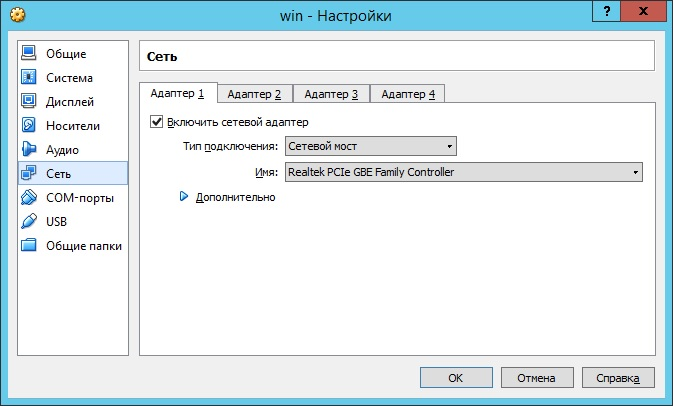
\includegraphics[width=.8\textwidth]{net_setup}\\
    Настройка сетевого адаптера виртуальной машины\\[2em]
    
    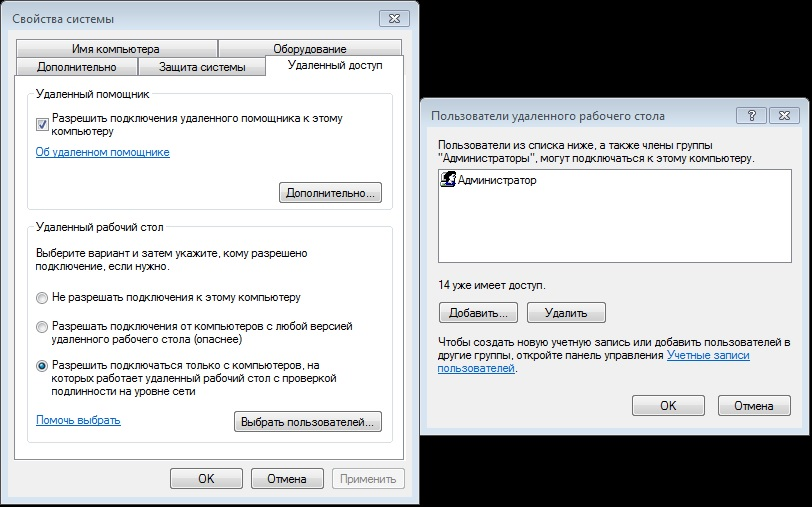
\includegraphics[width=.8\textwidth]{remote_access}\\
    Настройка удаленного доступа к виртуальной машине
  \end{figure}
  
  \newpage
  
  \begin{figure}[h!]
    \center
    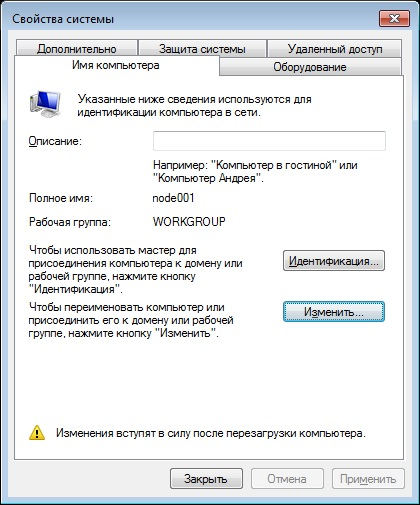
\includegraphics[width=.5\textwidth]{node001}\\
    Изменение имени виртуальной машины\\[2em]
    
    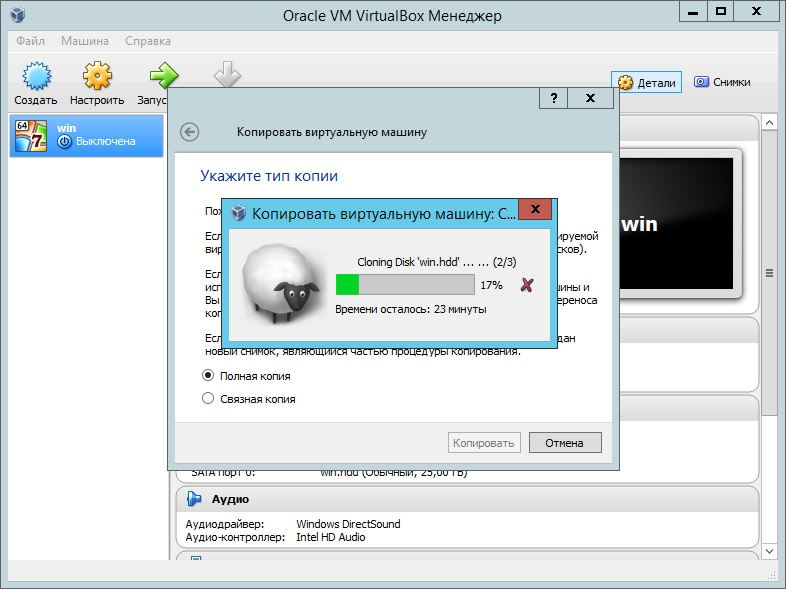
\includegraphics[width=.8\textwidth]{cloning}\\
    Клонирование виртуальной машины
  \end{figure}
  
  \newpage
  
  \begin{figure}[h!]
    \center
    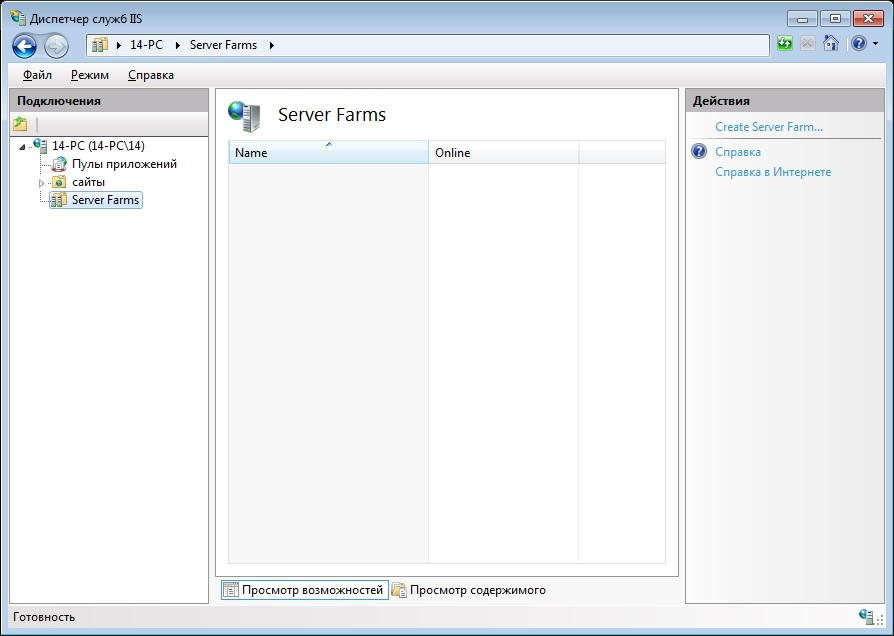
\includegraphics[width=.8\textwidth]{iis_wff_first}\\
    Настройка веб-фермы серверов (WFF)\\[2em]
    
    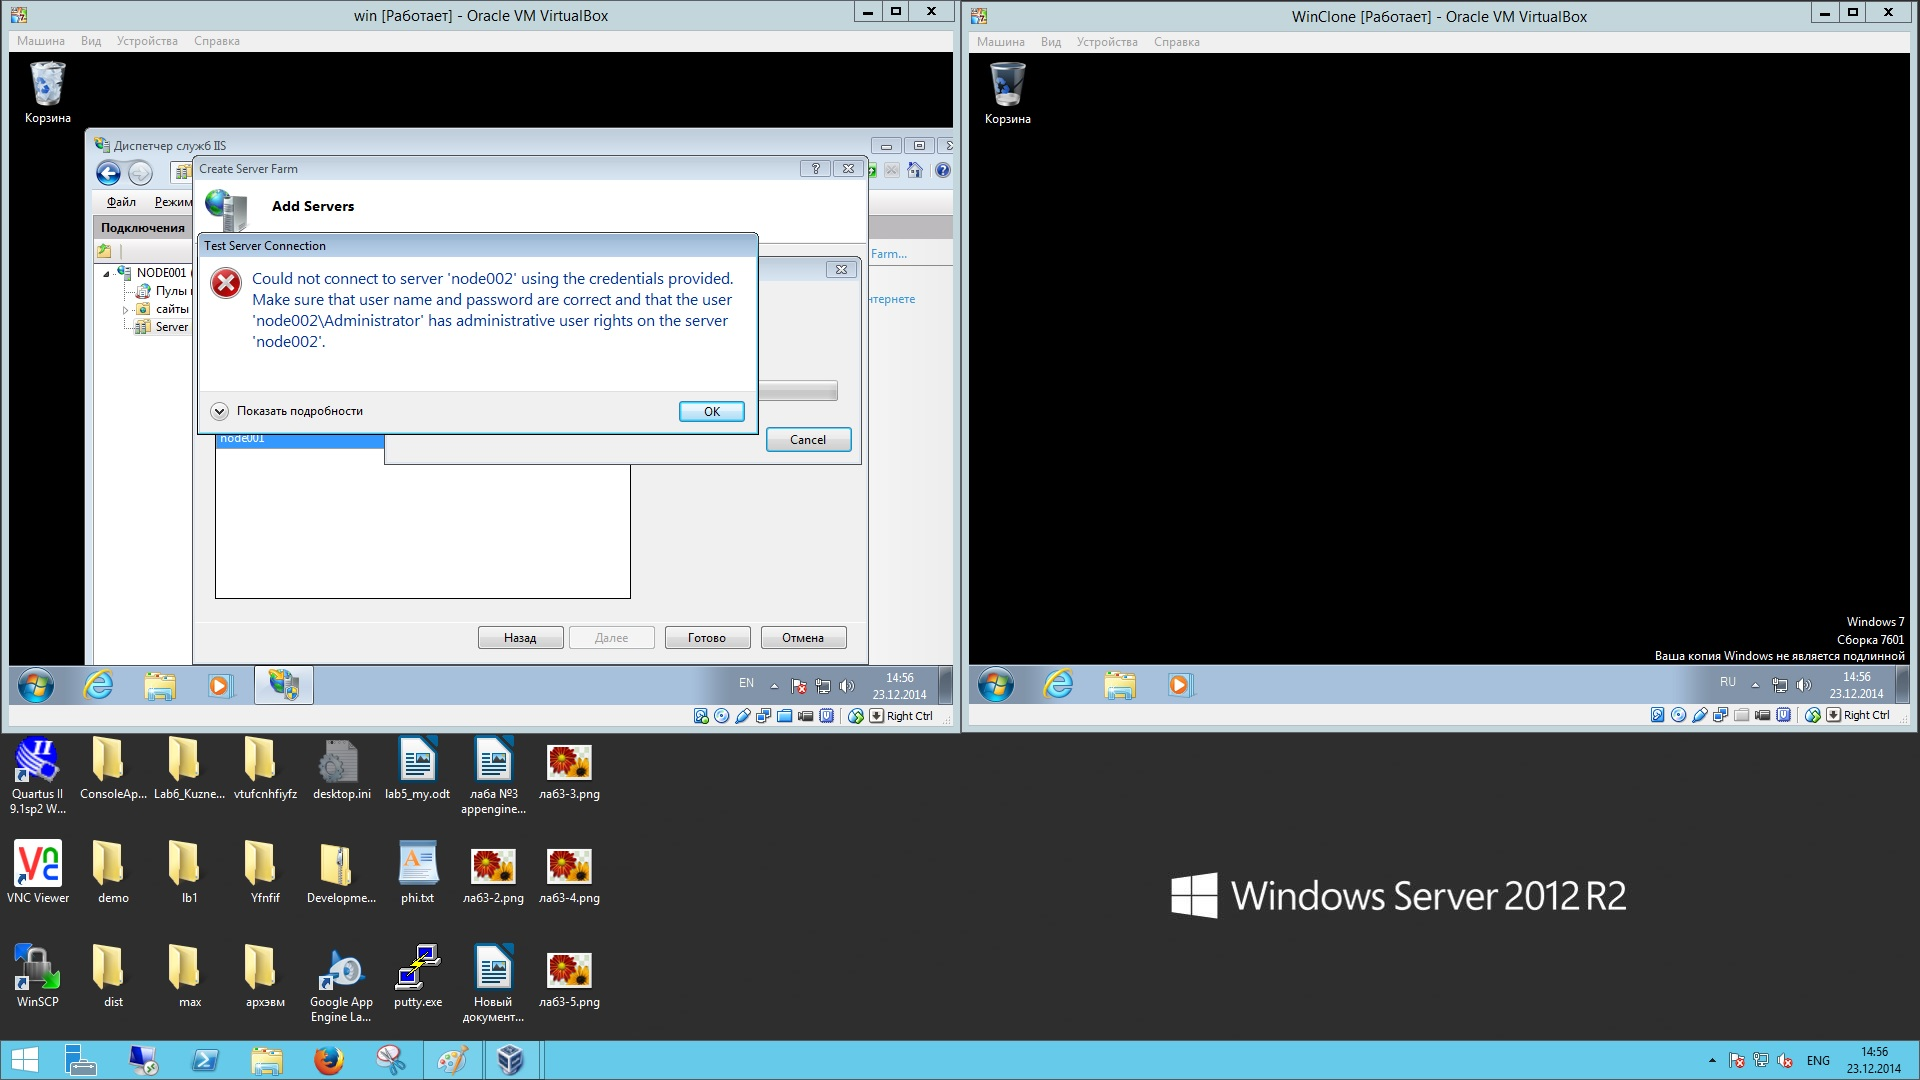
\includegraphics[width=.99\textwidth]{node002_fail}\\
    Попытка подключить второй узел по имени виртуальной машины
  \end{figure}
  
  \newpage
  
  \begin{figure}[h!]
    \center    
    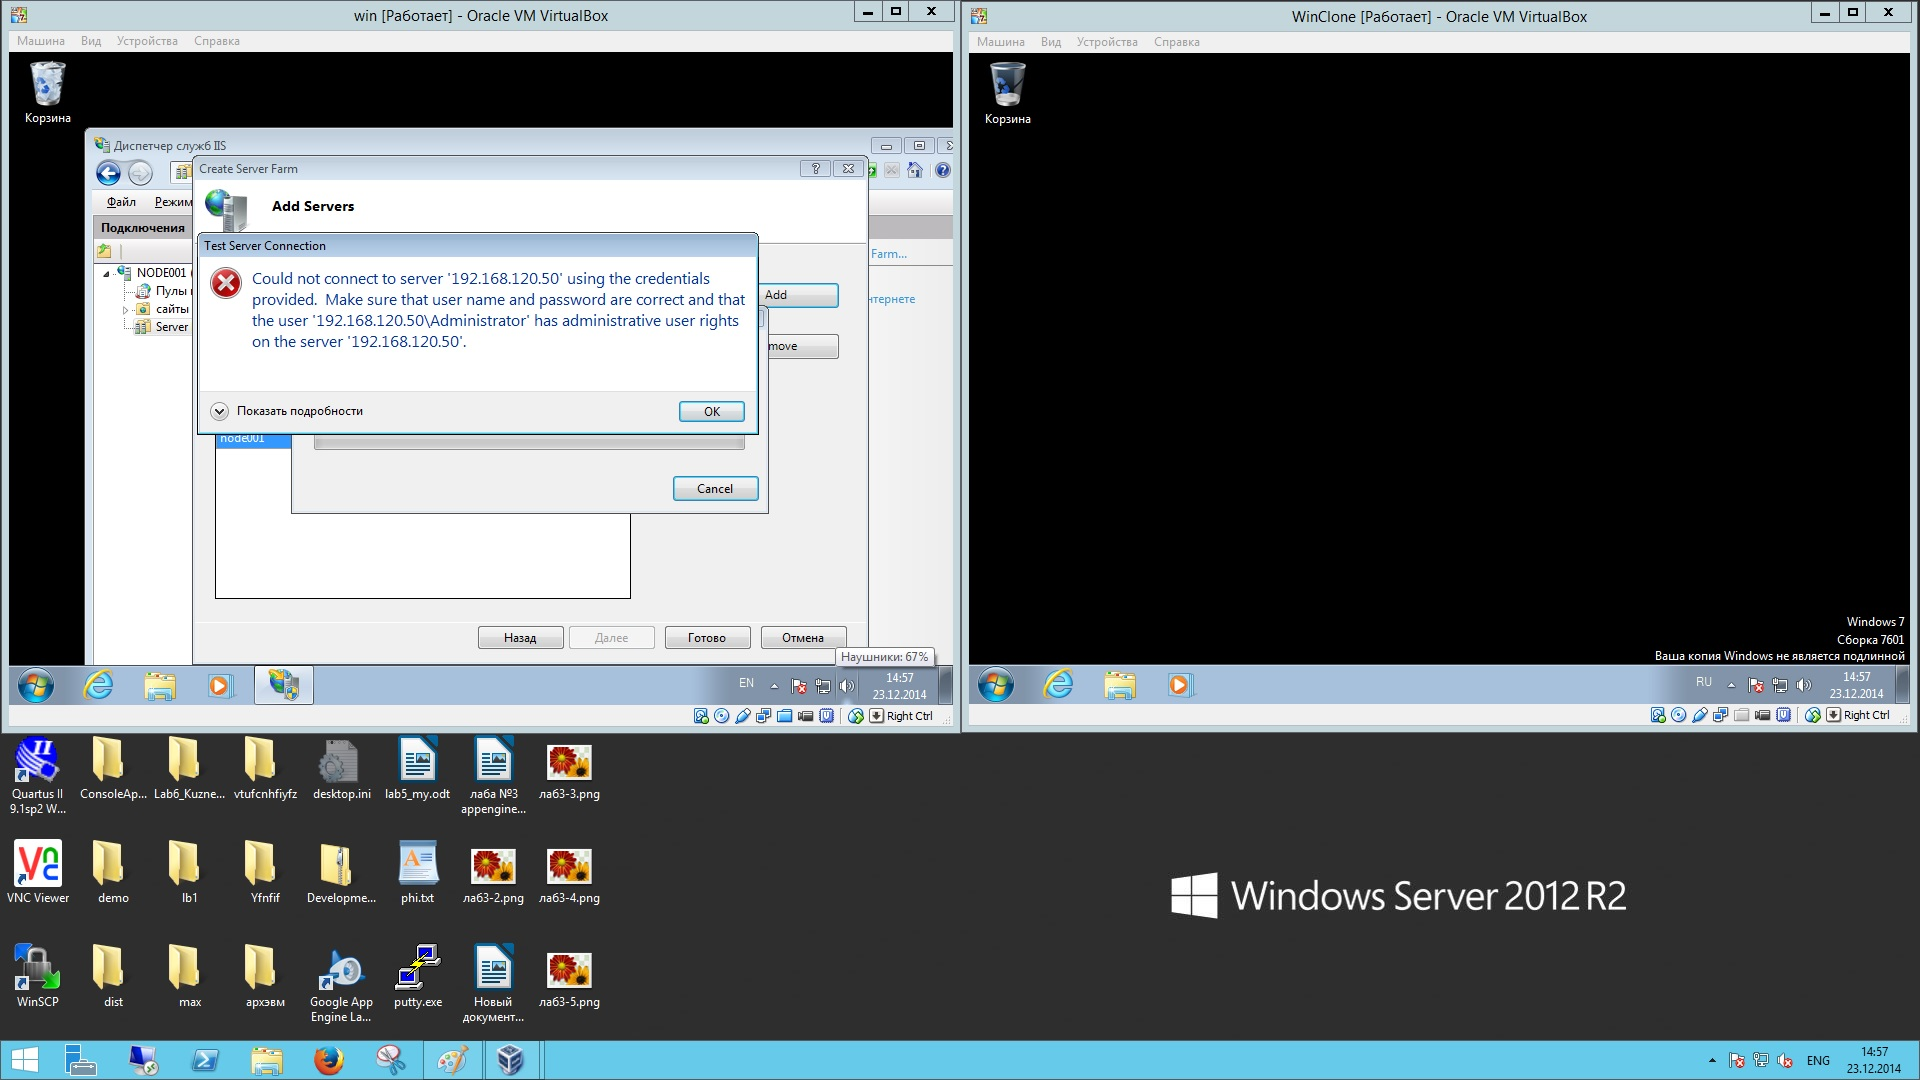
\includegraphics[width=.99\textwidth]{node002_fail2}\\
    Попытка подключить второй узел по IP-адресу виртуальной машины
  \end{figure}
  
\end{document}
